% SPDX-FileCopyrightText: © 2026 Idiap Research Institute <contact@idiap.ch>
%
% SPDX-FileContributor: Andre Freitas <andre.freitas@idiap.ch>
% Neuro-symbolic AI Group
%
% SPDX-FileContributor: Danilo Gusicuma <danilo.gusicuma@idiap.ch>
% Neuro-symbolic AI Group
%
% SPDX-License-Identifier: MIT
\documentclass[11pt]{article}

\usepackage[letterpaper,margin=1in]{geometry}
\usepackage[T1]{fontenc}
\usepackage{lmodern}
\usepackage{microtype}
\usepackage{amsmath,amssymb,amsthm,mathtools}
\usepackage{booktabs,array}
\usepackage{enumitem}
\usepackage{xcolor}
\usepackage{tikz}
\usetikzlibrary{arrows.meta,positioning,shapes.geometric,fit}
\usepackage[colorlinks=true,linkcolor=blue!55!black,citecolor=blue!55!black,urlcolor=blue!55!black]{hyperref}
\usepackage[nameinlink,capitalise,noabbrev]{cleveref}

\setlist[itemize]{leftmargin=*,itemsep=0.35em,topsep=0.35em}
\setlist[enumerate]{leftmargin=*,itemsep=0.35em,topsep=0.35em}
\allowdisplaybreaks

\newtheorem{theorem}{Theorem}[section]
\newtheorem{proposition}[theorem]{Proposition}
\newtheorem{lemma}[theorem]{Lemma}
\newtheorem{corollary}[theorem]{Corollary}
\theoremstyle{definition}
\newtheorem{definition}[theorem]{Definition}
\newtheorem{remark}[theorem]{Remark}
\newtheorem{openproblem}[theorem]{Open Problem}

\newcommand{\bits}{\{0,1\}}
\newcommand{\F}{\mathbb{F}_2}
\newcommand{\SIZE}{\operatorname{SIZE}}
\newcommand{\Ckt}{\operatorname{C}}
\newcommand{\SAT}{\mathrm{SAT}}
\newcommand{\Ppoly}{\mathrm{P/poly}}
\newcommand{\poly}{\operatorname{poly}}
\newcommand{\dist}{\operatorname{dist}}
\newcommand{\supp}{\operatorname{supp}}
\newcommand{\fr}{\operatorname{Forced}}
\newcommand{\Eq}{\operatorname{EQ}}
\newcommand{\eps}{\varepsilon}
\newcommand{\elln}{\ell_n}
\newcommand{\Mn}{M_n}
\newcommand{\Gn}{\mathbf{G}_n}
\newcommand{\Hsat}{H_n^{\SAT}}
\newcommand{\Hy}{H_n^y}
\newcommand{\Fz}{F_n^z}
\newcommand{\EqSAT}{\operatorname{EqSAT}}
\newcommand{\SemRows}{\operatorname{SemRows}}
\newcommand{\LinkRows}{\operatorname{LinkRows}}
\newcommand{\RowSupp}{\operatorname{RowSupp}}
\newcommand{\Cov}{\operatorname{Cov}}
\newcommand{\Ext}{\operatorname{Ext}}

\title{Parity Magnification and the Full-Row Barrier\\
\large From Exponent Debt to Certificate Debt in SAT Circuit Lower-Bound Transfers}
\author{Anonymous}
\date{}

\begin{document}
\maketitle

\begin{abstract}
A common hardness-magnification transfer has the form
\[
  \SAT\in\SIZE(m^c)\quad\Longrightarrow\quad
  \Ckt(H_n)\le n^{q+\beta c+o(1)}.
\]
A fixed source lower-bound exponent can rule out every polynomial SAT exponent only in the all-exponent regime $\beta=0$. We isolate this accounting principle and study a concrete $\beta=0$ carrier: the parity of $M_n=n^{q+o(1)}$ SAT instances of length $\ell_n=(\log n)^d$, generated by one batched circuit of size $n^{\rho+o(1)}$. If SAT has polynomial-size circuits, then the carrier has size $n^{\max\{q,\rho\}+o(1)}$. Thus an infinitely-often lower bound above $n^{1+\eps}$, for $\max\{q,\rho\}<1+\eps$, would imply $\SAT\notin\Ppoly$.

The main issue is then the proof of the source lower bound. We establish two obstructions for certificate-based approaches. First, a dense, truth-table-constructive certificate that is sound for every formula-labeling induces a Razborov--Rudich natural property useful against polynomial-size circuits. Second, an occurrence-relativizing certificate must force many complete aggregate rows. More generally, if a transcript is sound for all completions of the occurrence labels and claims circuit complexity greater than $s_n$, then it must query
\[
  \Omega\!\left((C_0(A_{M_n})+C_1(A_{M_n}))\frac{s_n}{n}\right)
\]
occurrences, where $C_b(A_{M_n})$ is the $b$-certificate complexity of the row aggregator. For parity, $C_0=C_1=M_n$, yielding an $\Omega(M_ns_n/n)$ query lower bound and, at $s_n=n^{1+\eps-o(1)}$, an $n^{q+\eps-o(1)}$ full-row barrier. The theorem applies to functional or occurrence-relativizing certificate systems. It does not cover proofs that exploit equality and semantic relations among repeated SAT formulas; that formula-semantic regime is the explicit nonrelativizing gap.

We refine that gap for concrete proof-system fragments. Pure occurrence extraction already fails for systems with an explicit $\EqSAT$ rule identifying equisatisfiable formulas: such a rule can determine parity through semantic links while forcing no complete occurrence row. The repaired invariant is not raw occurrence access but semantic row support. If a parsed proof determines all but $E_n$ rows by occurrence information and explicit semantic links, and the transcript plus residual circuit has size below the source threshold, then equality patching forces $E_n=\Omega(s_n/n)$. For witnessed extensionality rules, the same calculation gives a low-cover upper-bound falsifier: any proof whose equality and extensionality witnesses are uniformly openable with cover exponent $\alpha_{\mathrm{ext}}$ yields an upper bound
\[
  \Ckt(H_n^{\SAT})
  \le n^{\max\{\rho,q+\alpha_{\mathrm{ext}},\max\{f,r\}+1\}+o(1)}.
\]
Thus witnessed formula identity is harmless when the cover exponent is small; the remaining escape is an unwitnessed SAT-semantic principle for which no row-support or cover certificate is exposed.
\end{abstract}

\paragraph{Keywords.}
Circuit lower bounds; hardness magnification; natural proofs; certificate complexity; proof complexity; SAT; parity.

\section{Introduction}

Hardness magnification seeks a source problem for which a lower bound only slightly beyond the current frontier would imply a much stronger separation. The promise is quantitative: a modest source lower bound can be amplified through a carefully controlled reduction. The danger is quantitative as well. If the assumed target-circuit exponent survives inside the source upper bound, then a fixed source theorem excludes only a bounded range of target exponents.

This paper studies that tension in a simple SAT-to-circuit transfer. The first observation is an exponent ledger. Suppose that, for every fixed $c$,
\begin{equation}\label{eq:intro-ledger}
  \SAT\in\SIZE(m^c)
  \quad\Longrightarrow\quad
  \Ckt(H_n)\le n^{q+\beta c+o(1)}.
\end{equation}
A lower bound $\Ckt(H_n)>n^{a-o(1)}$ contradicts the assumption only when $a>q+\beta c$. If $\beta>0$, no fixed $a$ rules out all constants $c$. This is the \emph{exponent debt} of the transfer. The debt disappears when the target instances have subpolynomial length, and in particular when their length is polylogarithmic in $n$.

We therefore consider a batched generator
\[
  \Gn(x)=\bigl(G_{n,1}(x),\ldots,G_{n,\Mn}(x)\bigr),
  \qquad
  \ell_n=(\log n)^d,
  \qquad
  M_n=n^{q+o(1)},
\]
whose entire multi-output computation has size $n^{\rho+o(1)}$. The SAT parity carrier is
\begin{equation}\label{eq:intro-carrier}
  H_n^{\SAT}(x)
  =\bigoplus_{j=1}^{M_n}\SAT\bigl(G_{n,j}(x)\bigr).
\end{equation}
If SAT on $\ell_n$-bit inputs has circuits of size $\ell_n^c$, then substituting a copy into every slot gives
\[
  \Ckt(H_n^{\SAT})
  \le n^{\rho+o(1)}+n^{q+o(1)}\ell_n^c
  =n^{\max\{\rho,q\}+o(1)}.
\]
The exponent $c$ has vanished. Consequently, an infinitely-often lower bound $\Ckt(H_n^{\SAT})>n^{1+\eps}$ implies $\SAT\notin\Ppoly$ whenever $\max\{\rho,q\}<1+\eps$.

This transfer theorem is elementary. Its role is to identify exactly where the hard work moves. Once exponent debt has been eliminated, the remaining problem is to prove a barely superthreshold lower bound for the parity carrier. The central contribution of the paper is a classification of two broad certificate routes to that source lower bound.

\paragraph{Functional certificates.}
Let $y:\bits^{\ell_n}\to\bits$ be an arbitrary formula-labeling and define
\[
  H_n^y(x)=\bigoplus_{j\le M_n}y(G_{n,j}(x)).
\]
Suppose a property of $y$ is dense, decidable in time polynomial in the truth-table length $2^{\ell_n}$, and functionally sound in the sense that acceptance implies $\Ckt(H_n^y)>n^{1+\eps-o(1)}$ for every $y$. The $\beta=0$ transfer then makes the property useful against every fixed polynomial circuit size. It is therefore a natural property in the classical quantitative regime. The naturalization statement is unconditional; interpreting it as a barrier uses the usual pseudorandom-function hypothesis of Razborov and Rudich~\cite{RR97,GGM86}.

\paragraph{Occurrence-local certificates.}
A different proof may inspect only selected generated occurrences $(x,j)$ and remain sound under arbitrary completions of the uninspected occurrence labels. Such a transcript can be spoofed row by row. On every unforced row, complete the unseen labels so that the aggregate output is a fixed baseline. The resulting carrier differs from a constant on only the rows already forced by the transcript, and equality tests patch those rows at cost $O(n)$ each. Hence a certificate claiming complexity greater than $s_n$ must force $\Omega(s_n/n)$ rows.

The cost of forcing a row is governed by the ordinary certificate complexity of the aggregator. If $C_b(A_M)$ is the minimum number of input bits needed to force $A_M=b$, then full functional soundness gives the query lower bound
\begin{equation}\label{eq:intro-main}
  |Q|
  =\Omega\!\left((C_0(A_M)+C_1(A_M))\frac{s_n}{n}\right).
\end{equation}
For parity, $C_0=C_1=M$, so a forced row is a complete row. At the magnification threshold $s_n=n^{1+\eps-o(1)}$ and $M_n=n^{q+o(1)}$, every sound occurrence transcript must expose
\[
  n^{q+\eps-o(1)}
\]
occurrence labels.

\paragraph{Why parity.}
For an OR row, one positive label forces output $1$; for a parity row, either output requires all $M$ labels. Thus parity removes the cheap one-sided positive certificate that powers selector and separator compressions for generated OR carriers. Under full functional soundness OR also has an expensive negative side, but SAT-specific one-sided arguments need not expose it. Parity makes the full-row cost unavoidable even for one-sided forcing.

\paragraph{Scope and non-claims.}
The row-forcing theorem is a theorem about arbitrary occurrence labels. Actual SAT labels live in a much smaller structured set: equal formulas share labels, and formula syntax supports semantic relations such as self-reducibility. A proof system may exploit those relations to constrain many rows without reading their occurrences independently. We do not prove that full Extended Frege with SAT semantics reduces to the occurrence model, and we do not prove a lower bound for the explicit carrier in~\eqref{eq:intro-carrier}. The conclusion is a precise fork:
\begin{quote}
Dense functional certificates naturalize; occurrence-relativizing certificates pay full-row cost; a successful remaining route must use genuinely formula-semantic, nonrelativizing information or prove the lower bound directly.
\end{quote}

\paragraph{Semantic-link refinement.}
The fork can be made more concrete for proof systems that expose some of their SAT semantics. In an equality fragment with an explicit rule
\[
  \EqSAT(F,F'):\qquad F\simeq_{\mathrm{sat}} F'\ \Longrightarrow\ \SAT(F)=\SAT(F'),
\]
private occurrence completions are no longer admissible when they break the displayed equivalence. The correct repair is to charge rows covered by the proof's semantic links. A proof that covers too few rows still fails by the same sparse-row patching argument; a proof that covers many rows has paid certificate debt through semantics rather than through raw occurrence queries. For stronger systems the open issue becomes exact: either every SAT-semantic rule admits such a row-support/cover accounting, or the first rule that does not is the named nonrelativizing principle outside the present barrier.

\paragraph{Organization.}
\Cref{sec:model} fixes the circuit and carrier models. \Cref{sec:exponent} proves the exponent ledger and the $\beta=0$ transfer. \Cref{sec:patching} gives the sparse-row patching lemma. \Cref{sec:naturalization} proves the naturalization theorem. \Cref{sec:rowforcing} proves the general row-forcing and parity bounds. \Cref{sec:formula-v-occurrence} isolates the unresolved formula-semantic regime. \Cref{sec:semantic-links} adds the semantic-link and witnessed-extensionality refinements, and \Cref{sec:proof-systems} states proof-system consequences. An incidence-sketch upper-bound diagnostic appears in \Cref{app:incidence}.

\section{Model and notation}\label{sec:model}

\subsection{Circuit complexity}

We use nonuniform Boolean circuits over a fixed finite basis of fan-in two gates. XOR has constant-size implementations over the basis and is used freely with constant-factor overhead. For a Boolean function $f:\bits^n\to\bits$, let $\Ckt(f)$ denote its minimum circuit size. For a size function $s$, $\SIZE(s(n))$ is the class of languages having circuits of size $O(s(n))$ at length $n$, and
\[
  \Ppoly=\bigcup_{c\ge 1}\SIZE(n^c).
\]
All asymptotic statements allow constants depending on fixed parameters such as $c,d,q,$ and $\rho$. A statement holding infinitely often is abbreviated ``i.o.''

We fix a standard encoding of Boolean formulas. The predicate $\SAT_\ell:\bits^\ell\to\bits$ is defined on all strings of length $\ell$, with malformed encodings assigned value $0$.

\subsection{Batched generators and formula-label carriers}

\begin{definition}[Batched generator]\label{def:generator}
For each source length $n$, a batched generator is a multi-output circuit
\[
  \Gn:\bits^n\longrightarrow (\bits^{\ell_n})^{M_n},
  \qquad
  \Gn(x)=\bigl(G_{n,1}(x),\ldots,G_{n,M_n}(x)\bigr).
\]
Its size $g_n$ is the size of the single circuit producing all $M_n\ell_n$ output bits. The generator is \emph{label-independent}: its wiring and advice do not depend on the SAT truth table or on a later labeling $y$.
\end{definition}

The batched convention is important. If $n^\rho$ were the cost of generating one query rather than all queries, the transfer exponent would generally be $q+\rho$ rather than $\max\{q,\rho\}$.

Let $A_M:\bits^M\to\bits$ be a family of row aggregators having circuits of size $O(M)$. For a labeling $y:\bits^{\ell_n}\to\bits$, define the formula-label carrier
\begin{equation}\label{eq:formula-carrier}
  H_{n,A}^y(x)
  :=A_{M_n}\bigl(y(G_{n,1}(x)),\ldots,y(G_{n,M_n}(x))\bigr).
\end{equation}
The SAT carrier is $H_{n,A}^{\SAT}:=H_{n,A}^{\SAT_{\ell_n}}$. Unless otherwise stated, the main aggregator is parity,
\[
  A_M(z_1,\ldots,z_M)=z_1\oplus\cdots\oplus z_M,
\]
and we abbreviate $H_{n,\oplus}^y$ to $H_n^y$.

\subsection{Occurrence-label carriers}

Formula labels identify repeated formulas. To state the locality obstruction, we also use a relaxation in which every generated occurrence has an independent label.

\begin{definition}[Occurrence-label carrier]\label{def:occurrence-carrier}
Let
\[
  \Omega_n:=\bits^n\times[M_n].
\]
For an occurrence assignment $z:\Omega_n\to\bits$, define
\begin{equation}\label{eq:occurrence-carrier}
  F_{n,A}^z(x):=A_{M_n}\bigl(z(x,1),\ldots,z(x,M_n)\bigr).
\end{equation}
\end{definition}

Every formula labeling induces an occurrence assignment
\begin{equation}\label{eq:realization-map}
  z_y(x,j):=y(G_{n,j}(x)),
\end{equation}
but most occurrence assignments are not of this form. In particular, $z_y(x,j)=z_y(x',j')$ whenever the two generated formulas are identical. The row-forcing theorem applies to the larger occurrence space; \Cref{sec:formula-v-occurrence} explains why this distinction is the main scope boundary.

\subsection{Certificate complexity of the row aggregator}

A partial assignment $\alpha:S\to\bits$, $S\subseteq[M]$, \emph{forces} $A_M=b$ if every total string extending $\alpha$ has aggregator value $b$.

\begin{definition}[Aggregator certificate complexity]\label{def:cert-complexity}
For $b\in\bits$, let
\[
  C_b(A_M)
  :=\min\bigl\{|S|:\text{some partial assignment on }S\text{ forces }A_M=b\bigr\}.
\]
We also write $\kappa(A_M):=\min\{C_0(A_M),C_1(A_M)\}$.
\end{definition}

For parity, $C_0(\oplus_M)=C_1(\oplus_M)=M$. For OR, $C_1(\mathrm{OR}_M)=1$ while $C_0(\mathrm{OR}_M)=M$. These elementary values will explain the difference between one-sided OR evidence and parity evidence.

\section{Exponent debt and the beta-zero transfer}\label{sec:exponent}

We first separate a general accounting fact from the particular carrier.

\begin{proposition}[Exponent-window lemma]\label{prop:exponent-window}
Let $(H_n)$ be a Boolean-function family. Suppose there are constants $q,\beta\ge 0$ such that, for every fixed $c\ge 1$,
\begin{equation}\label{eq:general-transfer}
  \SAT\in\SIZE(m^c)
  \quad\Longrightarrow\quad
  \Ckt(H_n)\le n^{q+\beta c+o(1)}.
\end{equation}
If $\Ckt(H_n)>n^{a-o(1)}$ i.o., then
\[
  \SAT\notin\SIZE(m^c)
  \qquad\text{for every fixed }c\text{ satisfying }q+\beta c<a.
\]
Consequently, if $\beta>0$, one fixed source exponent $a$ excludes only a bounded interval of target exponents. If $\beta=0$ and $a>q$, it excludes every fixed polynomial exponent.
\end{proposition}

\begin{proof}
Fix $c$ with $q+\beta c<a$ and suppose $\SAT\in\SIZE(m^c)$. Choose $\delta>0$ such that
\[
  q+\beta c+2\delta<a.
\]
For all sufficiently large $n$, the transfer upper bound is at most $n^{q+\beta c+\delta}$, while on infinitely many sufficiently large $n$ the source lower bound exceeds $n^{a-\delta}$. These inequalities are incompatible. The final statements follow by solving $q+\beta c<a$ for $c$.
\end{proof}

The coefficient $\beta$ records the polynomial dependence of target query length on source length. If target queries have length $n^{\beta+o(1)}$, then substituting an $m^c$-size target circuit naturally contributes $n^{\beta c+o(1)}$. Polylogarithmic query length corresponds to $\beta=0$.

\subsection{Substitution into a batched carrier}

\begin{lemma}[Batched substitution]\label{lem:substitution}
Let $A_M$ have circuit size $O(M)$, and let $y:\bits^{\ell_n}\to\bits$ have circuit size $s_n$. Then
\begin{equation}\label{eq:batched-substitution}
  \Ckt(H_{n,A}^y)
  \le g_n+M_n s_n+O(M_n).
\end{equation}
\end{lemma}

\begin{proof}
Compute all $M_n$ queries with the batched generator. Feed each query into a separate copy of the size-$s_n$ circuit for $y$, and apply the size-$O(M_n)$ aggregator circuit to the resulting bits. The generator is paid once.
\end{proof}

We now specialize to the polylogarithmic regime
\begin{equation}\label{eq:parameter-regime}
  \ell_n=\left\lceil(\log n)^d\right\rceil,
  \qquad
  M_n=n^{q+o(1)},
  \qquad
  g_n=n^{\rho+o(1)},
\end{equation}
where $d>1$ and $q,\rho\ge 0$ are fixed. The condition $d>1$ is not needed merely for substitution; it ensures that hardwiring the complete $\ell_n$-bit SAT truth table costs
\[
  2^{\ell_n}=n^{(\log n)^{d-1}+o(1)}=n^{\omega(1)},
\]
so exhaustive lookup is not automatically a barely superlinear upper bound.

\begin{theorem}[Beta-zero parity transfer]\label{thm:beta-zero-transfer}
Under~\eqref{eq:parameter-regime}, for every fixed $c\ge 1$,
\begin{equation}\label{eq:beta-zero-bound}
  \SAT\in\SIZE(m^c)
  \quad\Longrightarrow\quad
  \Ckt(H_n^{\SAT})
  \le n^{\max\{q,\rho\}+o(1)}.
\end{equation}
The same conclusion holds for every size-$O(M_n)$ aggregator.
\end{theorem}

\begin{proof}
Apply \Cref{lem:substitution} with $s_n=\ell_n^c$. Since $c$ and $d$ are fixed,
\[
  \ell_n^c=(\log n)^{dc+o(1)}=n^{o(1)}.
\]
Therefore
\[
  g_n+M_n\ell_n^c+O(M_n)
  =n^{\rho+o(1)}+n^{q+o(1)}
  =n^{\max\{q,\rho\}+o(1)}.
\]
\end{proof}

\begin{corollary}[Conditional magnification to $\SAT\notin\Ppoly$]\label{cor:magnification}
Suppose that for some $a>\max\{q,\rho\}$,
\[
  \Ckt(H_n^{\SAT})>n^{a-o(1)}
\]
holds infinitely often. Then $\SAT\notin\Ppoly$. In particular, if
\[
  \Ckt(H_n^{\SAT})>n^{1+\eps-o(1)}\quad\text{i.o.}
  \qquad\text{and}\qquad
  \max\{q,\rho\}<1+\eps,
\]
then $\SAT\notin\Ppoly$.
\end{corollary}

\begin{proof}
If $\SAT\in\Ppoly$, then $\SAT\in\SIZE(m^c)$ for some fixed $c$. \Cref{thm:beta-zero-transfer} gives a carrier upper bound $n^{\max\{q,\rho\}+o(1)}$, contradicting the assumed lower bound on the infinite hard-length set.
\end{proof}

The corollary is a bridge, not a source lower bound. The rest of the paper studies what a certificate for the source lower bound would have to accomplish.

\section{Sparse-row patching and residual robustness}\label{sec:patching}

A barely superlinear exact lower bound is sensitive to approximators that fail on very few inputs. The following elementary lemma quantifies the sensitivity.

\begin{lemma}[Equality patching]\label{lem:equality-patching}
Let $f,g:\bits^n\to\bits$, and let
\[
  R:=\{x\in\bits^n:f(x)\ne g(x)\}.
\]
Then
\begin{equation}\label{eq:patching}
  \Ckt(f)\le \Ckt(g)+O(n|R|+|R|).
\end{equation}
\end{lemma}

\begin{proof}
For each $r\in R$, compute the equality predicate
\[
  \Eq_r(x)=\bigwedge_{i=1}^n
  \begin{cases}
    x_i,&r_i=1,\\
    \neg x_i,&r_i=0.
  \end{cases}
\]
using $O(n)$ gates. Let $R'\subseteq R$ contain precisely the rows for which the output of $g$ must be flipped. Because the equality predicates are mutually exclusive,
\[
  f(x)=g(x)\oplus\bigoplus_{r\in R'}\Eq_r(x).
\]
The correction circuit has size $O(n|R|+|R|)$.
\end{proof}

\begin{corollary}[Residual threshold]\label{cor:residual-threshold}
If $\Ckt(f)>s_n$, then every circuit $g$ of size $t_n<s_n$ must satisfy
\begin{equation}\label{eq:error-lower-bound}
  \dist(f,g)
  :=|\{x:f(x)\ne g(x)\}|
  =\Omega\!\left(\frac{s_n-t_n}{n}\right).
\end{equation}
In particular, a lower bound $\Ckt(f)>n^{1+\eps-o(1)}$ rules out every subthreshold circuit that errs on only $n^{\eps-o(1)}$ rows.
\end{corollary}

The patching lemma is the bridge from local proof information to circuit size. A certificate that controls too few source rows is compatible with a function supported on those rows, and such a function is cheap to hardwire.

\section{Functional certificates naturalize}\label{sec:naturalization}

We next formalize the first branch of the certificate fork. Let
\[
  \mathcal{B}_{\ell}:=\{y:\bits^{\ell}\to\bits\}
\]
denote the set of Boolean functions on $\ell$ input bits, represented by their full truth tables.

\begin{definition}[Functional label property]\label{def:functional-property}
A property $\mathcal{P}_n\subseteq\mathcal{B}_{\ell_n}$ is \emph{functionally sound at threshold $s_n$} for the carrier $H_n^y$ if
\begin{equation}\label{eq:functional-soundness}
  y\in\mathcal{P}_n
  \quad\Longrightarrow\quad
  \Ckt(H_n^y)>s_n
\end{equation}
for every labeling $y:\bits^{\ell_n}\to\bits$.
\end{definition}

The quantifier over every $y$ is decisive. Soundness only for the actual SAT labeling is a semantic statement and does not define a useful property of arbitrary truth tables.

\begin{definition}[Constructivity and largeness]\label{def:natural-quantities}
The property sequence $(\mathcal{P}_n)$ is
\begin{itemize}
  \item \emph{truth-table constructive} if membership in $\mathcal{P}_n$ is decidable in time $2^{O(\ell_n)}$, polynomial in the truth-table length $2^{\ell_n}$; and
  \item \emph{large} if there is a constant $K$ such that
  \[
    \Pr_{y\leftarrow\mathcal{B}_{\ell_n}}[y\in\mathcal{P}_n]
    \ge 2^{-K\ell_n}
  \]
  for all relevant $n$.
\end{itemize}
\end{definition}

A certificate relation $V_n(y,\pi)$ with $|\pi|=O(\ell_n)$ and verification time $2^{O(\ell_n)}$ is searchable within $2^{O(\ell_n)}$ time by exhaustive enumeration of $\pi$. More generally, the theorem below only needs constructivity of the accepted property itself.

\begin{theorem}[Naturalization of functional certificates]\label{thm:naturalization}
Assume~\eqref{eq:parameter-regime}. Let $s_n=n^{a-o(1)}$ for some $a>\max\{q,\rho\}$. If $(\mathcal{P}_n)$ is functionally sound at threshold $s_n$, truth-table constructive, and large, then $(\mathcal{P}_n)$ is a constructive large property useful against polynomial-size circuits on the matched input lengths $\ell_n$. Concretely, for every fixed $c$ and all sufficiently large relevant $n$,
\begin{equation}\label{eq:usefulness}
  y\in\mathcal{P}_n
  \quad\Longrightarrow\quad
  \Ckt(y)>\ell_n^c.
\end{equation}
\end{theorem}

\begin{proof}
Fix $c$. Suppose $y\in\mathcal{P}_n$ and $\Ckt(y)\le\ell_n^c$. By \Cref{lem:substitution},
\[
  \Ckt(H_n^y)
  \le n^{\rho+o(1)}+n^{q+o(1)}\ell_n^c
  =n^{\max\{q,\rho\}+o(1)}.
\]
Since $a>\max\{q,\rho\}$, the right-hand side is smaller than $s_n$ for all sufficiently large $n$, contradicting functional soundness. Thus the property is useful against circuits of size $\ell_n^c$ for every fixed $c$. Constructivity and largeness are assumptions, so the three natural-property conditions hold.
\end{proof}

\begin{corollary}[Conditional natural-proofs obstruction]\label{cor:natural-barrier}
Under the standard exponentially secure pseudorandom-function hypothesis used in the natural-proofs framework, no property satisfying the hypotheses of \Cref{thm:naturalization} can exist for a cofinal matched-length sequence.
\end{corollary}

\begin{proof}[Justification]
\Cref{thm:naturalization} produces a large, truth-table-constructive property useful against every fixed polynomial circuit size. The Razborov--Rudich argument rules out such properties under the stated pseudorandomness hypothesis~\cite{RR97,GGM86}.
\end{proof}

\begin{remark}[Certificates over a generated range]\label{rem:cylinder}
A certificate may formally use only labels on the generated formula set
\[
  U_n:=\{G_{n,j}(x):x\in\bits^n,\ j\in[M_n]\}.
\]
If an accepted subset of $\bits^{U_n}$ has density $\delta_n$, its cylinder extension to complete truth tables has exactly the same density: every assignment on $U_n$ has $2^{2^{\ell_n}-|U_n|}$ extensions. Thus sparsity of the realization image inside the space of source truth tables is not by itself an escape. The real escapes are failure of functional soundness, failure of truth-table constructivity, or accepted density below the naturalness threshold.
\end{remark}

\section{Occurrence-local certificates and the full-row barrier}\label{sec:rowforcing}

We now turn to certificates whose accepted transcript reads selected occurrence labels. The model is deliberately abstract: it captures any deterministic oracle verifier after fixing an accepted certificate and the resulting query-answer transcript.

\subsection{Accepted transcripts and forced rows}

Let $A_M$ be a fixed aggregator. A partial occurrence assignment is a pair $(Q,\alpha)$ where
\[
  Q\subseteq\Omega_n=\bits^n\times[M_n],
  \qquad
  \alpha:Q\to\bits.
\]
A total occurrence assignment $z$ \emph{extends} $(Q,\alpha)$ if $z|_Q=\alpha$.

For a row $x$, write
\[
  Q_x:=\{j:(x,j)\in Q\},
  \qquad
  \alpha_x:=\alpha|_{\{x\}\times Q_x}.
\]

\begin{definition}[Forced rows]\label{def:forced-rows}
For $b\in\bits$, define
\[
  R_b(Q,\alpha)
  :=\{x\in\bits^n:\alpha_x\text{ forces }A_{M_n}=b\}.
\]
The set of all forced rows is
\[
  R_*(Q,\alpha):=R_0(Q,\alpha)\cup R_1(Q,\alpha).
\]
\end{definition}

\begin{definition}[Completion soundness]\label{def:completion-soundness}
A partial transcript $(Q,\alpha)$ is \emph{$s_n$-sound under occurrence completions} if every total $z$ extending $(Q,\alpha)$ satisfies
\begin{equation}\label{eq:completion-soundness}
  \Ckt(F_{n,A}^z)>s_n.
\end{equation}
\end{definition}

If a deterministic oracle verifier accepts after asking the queries $Q$ and receiving the answers $\alpha$, then every oracle extending $\alpha$ produces the same transcript. Therefore any verifier whose acceptance is claimed to certify the lower bound for arbitrary occurrence oracles must make the accepted transcript completion-sound.

\subsection{The row-forcing theorem}

\begin{theorem}[Row-forcing theorem]\label{thm:row-forcing}
There is an absolute constant $c>0$ such that the following holds. Let $(Q,\alpha)$ be $s_n$-sound under occurrence completions, with $s_n\ge cn$. Then, for each $b\in\bits$,
\begin{equation}\label{eq:forced-output-rows}
  |R_b(Q,\alpha)|=\Omega\!\left(\frac{s_n}{n}\right).
\end{equation}
Consequently,
\begin{equation}\label{eq:query-lower-general}
  |Q|
  \ge C_0(A_{M_n})|R_0(Q,\alpha)|
      +C_1(A_{M_n})|R_1(Q,\alpha)|
  =\Omega\!\left(
      (C_0(A_{M_n})+C_1(A_{M_n}))\frac{s_n}{n}
    \right).
\end{equation}
\end{theorem}

\begin{proof}
Fix $b\in\bits$. We construct a total occurrence assignment $z^{(b)}$ extending $(Q,\alpha)$ such that
\begin{equation}\label{eq:baseline-completion}
  F_{n,A}^{z^{(b)}}(x)=1-b
  \qquad\text{for every }x\notin R_b(Q,\alpha).
\end{equation}
Consider a row $x\notin R_b(Q,\alpha)$. If $\alpha_x$ forces $A_{M_n}=1-b$, every completion has the desired value. Otherwise $\alpha_x$ is unforced, so there exists a completion of that row with output $1-b$. Because occurrence labels from different rows are independent, choose such a completion separately for every row. Rows in $R_b$ necessarily output $b$ under every completion.

Thus $F_{n,A}^{z^{(b)}}$ differs from the constant function $1-b$ only on the set $R_b(Q,\alpha)$. By \Cref{lem:equality-patching},
\[
  \Ckt(F_{n,A}^{z^{(b)}})
  \le O(1)+O(n|R_b(Q,\alpha)|).
\]
Completion soundness forces this quantity to exceed $s_n$, proving~\eqref{eq:forced-output-rows}.

Finally, every row in $R_b(Q,\alpha)$ contains at least $C_b(A_{M_n})$ queried coordinates by the definition of certificate complexity. The row sets are disjoint, and summing the queried coordinates over rows gives~\eqref{eq:query-lower-general}.
\end{proof}

The proof is a private-row spoof. It leaves the observed transcript untouched, but uses one or more unseen labels in every unforced row to collapse the carrier to a constant outside the forced rows. Equality patching then converts row locality into a circuit upper bound.

A weaker but sometimes more intuitive consequence uses only the minimum forcing cost.

\begin{corollary}[Minimum-certificate form]\label{cor:min-cert-form}
Under the hypotheses of \Cref{thm:row-forcing},
\[
  |R_*(Q,\alpha)|=\Omega(s_n/n)
  \qquad\text{and}\qquad
  |Q|=\Omega\!\left(\kappa(A_{M_n})\frac{s_n}{n}\right).
\]
\end{corollary}

\subsection{Parity and OR}

\begin{corollary}[Full-row barrier for parity]\label{cor:parity-full-row}
For the parity aggregator, every $s_n$-sound occurrence transcript satisfies
\begin{equation}\label{eq:parity-query-lower}
  |Q|=\Omega\!\left(M_n\frac{s_n}{n}\right).
\end{equation}
In particular, if
\[
  M_n=n^{q+o(1)}
  \qquad\text{and}\qquad
  s_n=n^{1+\eps-o(1)},
\]
then
\begin{equation}\label{eq:parity-threshold}
  |Q|\ge n^{q+\eps-o(1)}.
\end{equation}
Moreover, every row counted in $R_0\cup R_1$ is complete: all $M_n$ labels in that row belong to $Q$.
\end{corollary}

\begin{proof}
A proper partial assignment to parity leaves at least one free bit, whose flip changes the output. Hence $C_0(\oplus_{M_n})=C_1(\oplus_{M_n})=M_n$. Substitute these values into \Cref{thm:row-forcing}.
\end{proof}

The contrast with OR is useful but must be stated carefully.

\begin{center}
\begin{tabular}{@{}lccc@{}}
\toprule
Aggregator $A_M$ & $C_1(A_M)$ & $C_0(A_M)$ & Cost to force one positive row \\
\midrule
$\mathrm{OR}_M$ & $1$ & $M$ & one positive occurrence \\
$\oplus_M$ & $M$ & $M$ & the entire row \\
\bottomrule
\end{tabular}
\end{center}

A one-sided OR certificate can expose a positive row with one witness. This is the structural source of selector, separator, and positive-cover upper bounds for generated OR carriers. Under the full completion-soundness hypothesis, \Cref{thm:row-forcing} also demands many forced zero rows for OR and therefore many full negative rows. But SAT-specific one-sided methods generally do not satisfy functional soundness over arbitrary occurrence completions. Parity is stronger for the present purpose because even the positive side has certificate complexity $M$.

\subsection{Adaptive verifiers}

\begin{corollary}[Oracle-query lower bound]\label{cor:oracle-verifier}
Let $V$ be a deterministic verifier that, on a fixed certificate $\pi$ and an occurrence oracle $z$, adaptively queries occurrence labels and accepts. Suppose acceptance is sound in the following functional sense:
\[
  V^z(\pi)=1
  \quad\Longrightarrow\quad
  \Ckt(F_{n,A}^z)>s_n
  \qquad\text{for every occurrence oracle }z.
\]
Then every accepted execution makes
\[
  \Omega\!\left((C_0(A_{M_n})+C_1(A_{M_n}))\frac{s_n}{n}\right)
\]
oracle queries. For parity at the magnification threshold, this is $n^{q+\eps-o(1)}$.
\end{corollary}

\begin{proof}
Fix an accepted execution and let $(Q,\alpha)$ be its query-answer transcript. Any oracle extending $\alpha$ produces the same adaptive execution, because every query asked along the path receives the same answer. Functional soundness makes the transcript completion-sound, so \Cref{thm:row-forcing} applies.
\end{proof}

\section{Formula labels versus occurrence labels}\label{sec:formula-v-occurrence}

The source carrier uses formula labels, while the row-forcing theorem allows occurrence labels to vary independently. The distinction is not cosmetic.

Define the occurrence-to-formula map
\[
  \Phi_n:\Omega_n\to\bits^{\ell_n},
  \qquad
  \Phi_n(x,j)=G_{n,j}(x).
\]
The formula-realizable occurrence assignments are exactly those of the form $z=y\circ\Phi_n$. They obey all equality constraints
\begin{equation}\label{eq:collision-constraints}
  \Phi_n(x,j)=\Phi_n(x',j')
  \quad\Longrightarrow\quad
  z(x,j)=z(x',j').
\end{equation}
The SAT assignment obeys additional semantic relations among different formulas. A private-row completion used in \Cref{thm:row-forcing} will usually violate~\eqref{eq:collision-constraints}: the unseen occurrence flipped in one row may be a formula already present in many other rows.

This yields three distinct certificate regimes.

\begin{figure}[t]
\centering
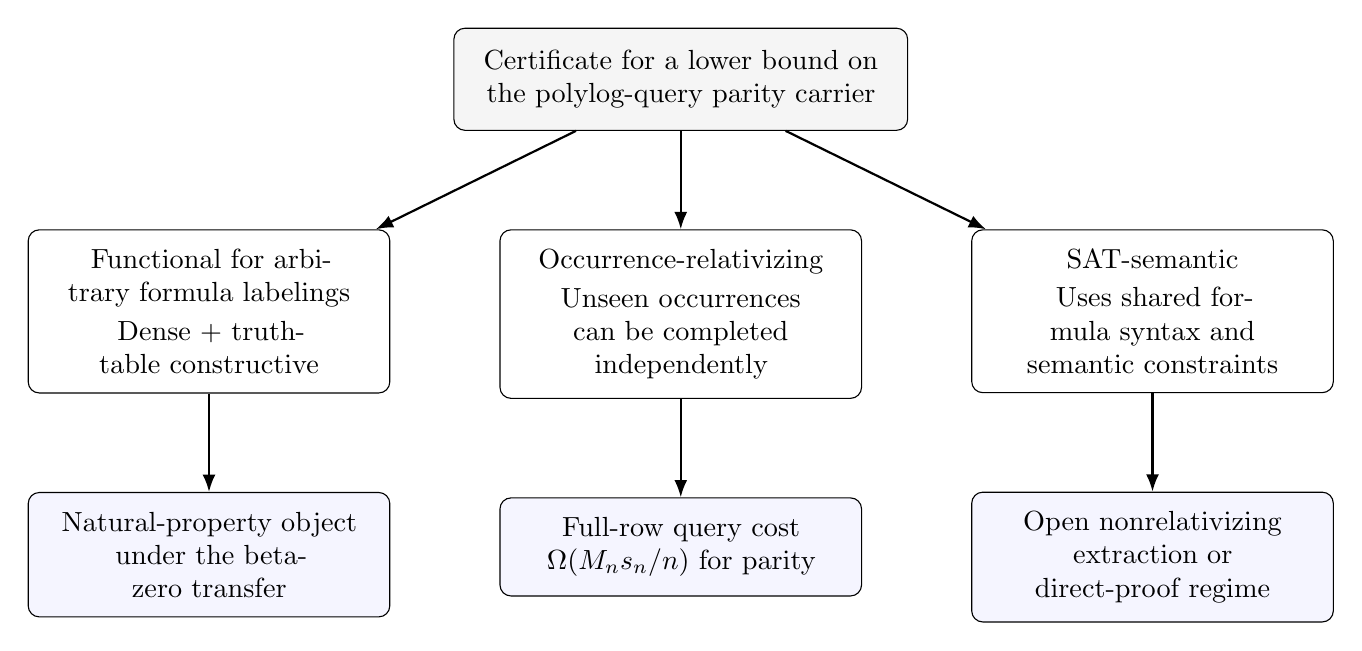
\begin{tikzpicture}[
  node distance=1.25cm and 0.8cm,
  box/.style={draw,rounded corners,align=center,inner sep=7pt,text width=4.1cm},
  top/.style={draw,rounded corners,align=center,inner sep=8pt,text width=5.2cm,fill=gray!8},
  arr/.style={-{Latex[length=2.2mm]},thick}
]
\node[top] (source) {Certificate for a lower bound on the polylog-query parity carrier};
\node[box,below left=of source] (functional) {Functional for arbitrary formula labelings\\[2pt]
Dense + truth-table constructive};
\node[box,below=of source] (occ) {Occurrence-relativizing\\[2pt]
Unseen occurrences can be completed independently};
\node[box,below right=of source] (semantic) {SAT-semantic\\[2pt]
Uses shared formula syntax and semantic constraints};
\node[box,below=of functional,fill=blue!4] (nat) {Natural-property object\\under the beta-zero transfer};
\node[box,below=of occ,fill=blue!4] (row) {Full-row query cost\\$\Omega(M_ns_n/n)$ for parity};
\node[box,below=of semantic,fill=blue!4] (open) {Open nonrelativizing\\extraction or direct-proof regime};
\draw[arr] (source) -- (functional);
\draw[arr] (source) -- (occ);
\draw[arr] (source) -- (semantic);
\draw[arr] (functional) -- (nat);
\draw[arr] (occ) -- (row);
\draw[arr] (semantic) -- (open);
\end{tikzpicture}
\caption{The certificate fork. The first two branches are covered by the theorems in this paper. The third is the explicit unresolved regime.}
\label{fig:fork}
\end{figure}

\begin{enumerate}
  \item A certificate that is sound for every formula labeling $y$ can be tested as a property of truth tables. If it is dense and constructive, \Cref{thm:naturalization} applies.
  \item A certificate whose transcript and soundness relativize to arbitrary occurrence labels is subject to \Cref{thm:row-forcing}.
  \item A certificate may be sound only for the actual SAT labeling and may derive consequences from formula syntax, equality, or self-reducibility. Such a proof need not define a useful property of arbitrary labelings and need not be invariant under occurrence-wise spoofing.
\end{enumerate}

The third regime is not a loophole in either proof; it violates their hypotheses. It is also the exact regime that must be understood before applying the row-forcing theorem to a strong proof system with SAT axioms.

\begin{openproblem}[Formula-semantic extraction]\label{op:semantic-extraction}
For a concrete strong proof system formalizing lower bounds for $H_n^{\SAT}$, prove one of the following:
\begin{enumerate}[label=(\alph*)]
  \item accepted short proofs induce dense constructive properties that are functionally sound over formula labelings;
  \item accepted short proofs admit occurrence-relativizing transcripts with quantitatively bounded query sets; or
  \item neither extraction is possible because the proof uses a precisely identified nonrelativizing SAT-semantic principle.
\end{enumerate}
\end{openproblem}

A solution of part (a) would connect the proof to naturalization. A solution of part (b) would convert \Cref{cor:parity-full-row} into a proof-size or oracle-query lower bound. Part (c) would isolate the semantic ingredient a successful magnification proof must exploit.

\section{Semantic links and witnessed extensionality}\label{sec:semantic-links}

The previous section leaves the formula-semantic branch open. We now record two refinements of that branch. They are deliberately modest. They do not give a lower bound for Extended Frege, but they sharpen the obstruction: some semantic proof steps can be charged as row support, while uncharged semantic steps are precisely the remaining nonrelativizing escape.

\subsection{Equality links are not occurrence queries}

Consider a proof system fragment, denoted here by $\mathcal{S}_{=}$, consisting of propositional reasoning over displayed SAT atoms together with explicit sound equality links
\[
  \EqSAT(F,F'):\qquad F\simeq_{\mathrm{sat}}F'\Longrightarrow \SAT(F)=\SAT(F'),
\]
where $F\simeq_{\mathrm{sat}}F'$ is a syntactically checkable equisatisfiability transformation such as padding, renaming, duplicate-clause insertion, or a displayed definitional extension. Such a rule is harmless for soundness, but it is fatal to a pure occurrence parser: a proof may determine parity by linking formulas, not by querying both occurrences independently.

\begin{proposition}[Occurrence-only extraction fails for equality fragments]\label{prop:eqsat-occurrence-failure}
There are beta-zero parity carriers with repeated or padded formula pairs for which $\mathcal{S}_{=}$ derives row-parity cancellations through $\EqSAT$ links while no occurrence-only transcript forces the paired rows in the sense of \Cref{def:forced-rows}. Consequently, the parser hypothesis in \Cref{prop:parser} is false for $\mathcal{S}_{=}$ unless the parser records equality links as additional semantic information.
\end{proposition}

\begin{proof}
Let a row contain two parity positions generated as $F$ and $F'=\operatorname{Pad}(F)$, where padding preserves satisfiability and is checkable inside the proof system. The $\EqSAT(F,F')$ rule proves $\SAT(F)=\SAT(F')$, so the contribution
\[
  \SAT(F)\oplus \SAT(F')
\]
is determined to be $0$ without separately reading both occurrences as independent labels. A private occurrence completion that assigns different Boolean values to the two positions may preserve an occurrence-only transcript, but it violates the displayed equality link. Hence acceptance is not invariant under all occurrence oracles extending that transcript. This is exactly the invariance hypothesis required by \Cref{prop:parser}, so the occurrence-only parser is not a valid abstraction for $\mathcal{S}_{=}$.
\end{proof}

The failure is informative rather than destructive. It says that equality fragments should be audited by a semantic-link transcript rather than by raw occurrence access.

\begin{definition}[Semantic-link residual transcript]\label{def:semantic-link-transcript}
Fix a proof system fragment $\mathcal{S}$ and a proof $\pi$ of a lower-bound statement for $\Hsat$. A semantic-link residual transcript consists of
\[
  T_\pi=(Q_\pi,\alpha_\pi,E_\pi,R_\pi,D_\pi),
\]
where $(Q_\pi,\alpha_\pi)$ is the occurrence information used by the proof, $E_\pi$ is a set of displayed semantic links between generated SAT atoms or formulas, $R_\pi\subseteq\bits^n$ is a residual set of source rows, and $D_\pi$ is a circuit such that, assuming the displayed links in $E_\pi$ are sound,
\[
  D_\pi(x)=\Hsat(x)\qquad\text{for every }x\notin R_\pi .
\]
The transcript is \emph{advice-free} if $Q_\pi,E_\pi,R_\pi,D_\pi$ are obtained from the proof and the fixed generator without an additional hardwired truth table for $\SAT$ on the generated formulas.
\end{definition}

\begin{proposition}[Semantic-link residual gate]\label{prop:semantic-link-gate}
Let $\pi$ be an accepted certificate for the statement $\Ckt(\Hsat)>s_n$. Suppose $\pi$ admits an advice-free semantic-link residual transcript $T_\pi$ with residual circuit size $S_D=\Ckt(D_\pi)$ and residual set size $E_n=|R_\pi|$. Then
\begin{equation}\label{eq:semantic-link-upper}
  \Ckt(\Hsat)\le S_D+O(E_n n+E_n).
\end{equation}
In particular, if $s_n=n^{1+\eps-o(1)}$ and $S_D<n^{1+\eps-o(1)}$, soundness of the certificate requires
\begin{equation}\label{eq:semantic-link-threshold}
  E_n\ge n^{\eps-o(1)} .
\end{equation}
\end{proposition}

\begin{proof}
The circuit $D_\pi$ computes $\Hsat$ outside $R_\pi$. Patch the exceptional rows exactly as in \Cref{lem:equality-patching}: for each $r\in R_\pi$, hardwire the desired value and test $x=r$ using $O(n)$ gates. This gives~\eqref{eq:semantic-link-upper}. If $E_n<n^{\eps-o(1)}$ and $S_D<n^{1+\eps-o(1)}$, the right-hand side is below $n^{1+\eps-o(1)}$, contradicting the certified lower bound. Thus any sound certificate in this regime must leave at least $n^{\eps-o(1)}$ genuinely unpatchable rows, or else it is only a sparse residual certificate.
\end{proof}

For $\mathcal{S}_{=}$, the row charge should therefore be read as equality-link coverage rather than occurrence coverage. A proof that derives parity through many equality links has not evaded certificate debt; it has paid that debt through $\LinkRows(E_\pi)$ instead of through $Q_\pi$. The open problem is to prove that a richer proof system admits a complete semantic-link transcript, or to isolate the first rule for which no such transcript can be extracted.

\subsection{Composition and semantic row support}

Equality is not the only semantic dependency. A system with local SAT-composition axioms, for example
\[
  \SAT(F\lor G)=\SAT(F)\lor\SAT(G),
\]
may constrain rows through formulas that are not themselves generated occurrences. This motivates a row-support version of the previous gate.

\begin{definition}[Semantic row support]\label{def:semantic-row-support}
For a parsed proof $\pi$, assign each nonlogical SAT axiom instance $a$ a source-row support set $\RowSupp(a)\subseteq\bits^n$: generated atoms support the rows in which they occur; equality links preserve support; and composition axioms support the union of the generated leaves on which the composed formula depends. Let
\[
  K_\pi:=\bigcup_{a\in Ax_{\SAT}(\pi)}\RowSupp(a).
\]
\end{definition}

\begin{proposition}[Conditional semantic-support forcing]\label{prop:semantic-support-forcing}
Assume a proof system $\mathcal{S}_{\mathrm{comp}}$ has a parser satisfying the following semantic-completion property: for every accepted proof $\pi$ and every residual circuit $D$ agreeing with $\Hsat$ outside $K_\pi$, the proof remains sound in a completion that realizes $D$ on rows outside $K_\pi$ while preserving all parsed SAT axioms. If $\pi$ certifies $\Ckt(\Hsat)>s_n$ and $\Ckt(D)=S_D<s_n$, then
\[
  |K_\pi|=\Omega\!\left(\frac{s_n-S_D}{n}\right).
\]
In particular, at $s_n=n^{1+\eps-o(1)}$ with $S_D<n^{1+\eps-o(1)}$, a valid proof must have $|K_\pi|\ge n^{\eps-o(1)}$.
\end{proposition}

\begin{proof}
If $|K_\pi|=o((s_n-S_D)/n)$, patch $D$ on the rows in $K_\pi$ by equality tests. The resulting circuit computes $\Hsat$ and has size
\[
  S_D+O(n|K_\pi|+|K_\pi|)<s_n,
\]
contradicting the certified lower bound. The semantic-completion assumption is what permits this residual replacement without violating the proof's displayed SAT axioms.
\end{proof}

The assumption in \Cref{prop:semantic-support-forcing} is the real work. For equality-only fragments it is plausible because equality closure is explicit. For richer systems, a finite obstruction already appears: an axiom for $\SAT(F\lor G)$ can involve generated leaves from several rows without being captured by equality fibers alone. Thus equality-closed row charge is a theorem candidate for equality fragments, while composition fragments require a separate semantic-completion theorem.

\subsection{Witnessed extensionality gives a finite upper-bound test}

There is one further useful boundary. If formula-identity or extensionality rules come with explicit witnesses, then they can be charged quantitatively. Let $\mathcal{S}_{\mathrm{wExt}}$ be a fragment in which every extensionality line
\[
  \Ext(F,F',w)
\]
contains a checkable witness $w$ for a satisfiability-preserving transformation, quotient, or transducer from $F$ to $F'$.

\begin{definition}[Cover exponent]\label{def:cover-exponent}
Suppose a parser for a proof $\pi$ opens all occurrence queries, equality quotients, and witnessed extensionality lines by an advice-free protocol of cost
\[
  n^{\alpha_{\mathrm{ext}}+o(1)}.
\]
Let $F_\pi$ and $R_\pi$ be the forced and residual source-row sets, with
\[
  |F_\pi|\le n^{f+o(1)},\qquad |R_\pi|\le n^{r+o(1)}.
\]
\end{definition}

\begin{proposition}[Witnessed-extensionality cover bound]\label{prop:wext-cover}
For the beta-zero carrier with $M_n=n^{q+o(1)}$ and generator size $n^{\rho+o(1)}$, any proof in $\mathcal{S}_{\mathrm{wExt}}$ admitting the cover in \Cref{def:cover-exponent} yields
\begin{equation}\label{eq:wext-cover-bound}
  \Ckt(\Hsat)
  \le
  n^{\max\{\rho,\ q+\alpha_{\mathrm{ext}},\ \max\{f,r\}+1\}+o(1)} .
\end{equation}
Consequently, if the exponent on the right is strictly below $1+\eps$, such a proof cannot certify $\Ckt(\Hsat)>n^{1+\eps-o(1)}$.
\end{proposition}

\begin{proof}
Generate the $M_n$ query formulas at cost $n^{\rho+o(1)}$. On nonexceptional rows, evaluate the row parity using the cover opener for the quotient and witnessed-extensionality information. This costs $n^{q+\alpha_{\mathrm{ext}}+o(1)}$. Patch forced or residual rows by equality tests, at cost
\[
  O\!\left(n(|F_\pi|+|R_\pi|)\right)
  =
  n^{\max\{f,r\}+1+o(1)} .
\]
Taking the maximum of these contributions gives~\eqref{eq:wext-cover-bound}. If that bound is below the claimed lower-bound threshold, the claimed certificate is falsified in the same circuit model.
\end{proof}

This proposition separates two cases. Witnessed formula identity is not a mysterious escape; it becomes another cover cost in the upper-bound ledger. Unwitnessed semantic equality, self-reduction, or extensionality is different. If it cannot be represented by occurrence access, row support, or a low-cover witness, then it is exactly the nonrelativizing SAT-semantic principle demanded by \Cref{op:semantic-extraction}.

\section{Consequences for proof-mediated magnification}\label{sec:proof-systems}

The Cook--Reckhow framework treats a proof system as an efficiently verifiable certificate relation~\cite{CR79}. Our results do not establish lower bounds for Extended Frege or for any standard strong system. They give conditional consequences once a proof parser or oracle interpretation is supplied.

\begin{proposition}[Parser-to-query consequence]\label{prop:parser}
Suppose a proof system $\mathcal{S}$ has the following property for a family of statements asserting
\[
  \Ckt(F_{n,\oplus}^z)>s_n.
\]
From every accepted proof $\pi$, a deterministic parser extracts a partial occurrence transcript $(Q_\pi,\alpha_\pi)$ such that:
\begin{enumerate}[label=(\roman*)]
  \item acceptance is invariant under every occurrence oracle extending $(Q_\pi,\alpha_\pi)$; and
  \item soundness of the proof implies the claimed lower bound for every such extension.
\end{enumerate}
Then
\[
  |Q_\pi|=\Omega(M_ns_n/n).
\]
If every proof of length $T$ exposes at most $p(T,n)$ occurrences, then every accepted proof satisfies
\[
  p(T,n)=\Omega(M_ns_n/n).
\]
\end{proposition}

\begin{proof}
Conditions (i) and (ii) make the extracted transcript completion-sound. Apply \Cref{cor:parity-full-row}.
\end{proof}

For an explicit-query proof encoding with $|Q_\pi|=O(|\pi|)$, the proposition gives a linear proof-length lower bound of order $M_ns_n/n$. If a verifier can generate polynomially many oracle queries from a shorter proof, the conclusion should instead be read as a lower bound on the verifier's occurrence access, or inverted through the particular relation $p(T,n)$.

At the intended parameters,
\[
  M_n=n^{q+o(1)},
  \qquad
  s_n=n^{1+\eps-o(1)},
\]
the parser must account for $n^{q+\eps-o(1)}$ occurrence labels. This is the precise meaning of \emph{certificate debt}: eliminating the target exponent by using many polylogarithmic queries creates a large local-information burden for any occurrence-relativizing source proof.

A direct proof of the exact lower-bound statement $\Ckt(H_n^{\SAT})>s_n$ is not invalidated by the patching lemma. It automatically rules out all residual pairs $(D,R)$ with
\[
  \Ckt(D)+O(n|R|)<s_n.
\]
The issue is instead whether a purportedly weaker certificate really establishes that exact statement, or merely supplies local SAT evidence that is compatible with an easy completion.

\paragraph{Semantic proof fragments.}
\Cref{sec:semantic-links} refines the interpretation of the parser hypothesis. For equality fragments, pure occurrence extraction is too strong and therefore false; equality links must be charged as semantic row support. For witnessed extensionality fragments, low-cover witnesses feed directly into the upper-bound ledger~\eqref{eq:wext-cover-bound}. Thus the proof-system consequence is no longer merely ``find a parser''; it is:
\begin{quote}
either extract functional soundness, extract occurrence access, extract semantic row support with enough charge, or identify an uncharged SAT-semantic principle.
\end{quote}
This is the concrete content of the formula-semantic fork.

\section{Related work}\label{sec:related}

\paragraph{Hardness magnification.}
Hardness magnification for natural problems was developed as a way to derive major circuit lower bounds from lower bounds near current frontiers~\cite{OS18,OPS19}. Chen, Hirahara, Oliveira, Pich, Rajgopal, and Santhanam studied the interaction of magnification with natural proofs and locality, including barriers to localizable lower-bound methods~\cite{CHOPRS19}. The present work is narrower. It isolates an exponent-accounting condition for an all-polynomial-exponent SAT transfer and studies certificate locality for one polylog-query parity carrier. It does not provide the required source lower bound.

\paragraph{Natural proofs.}
Razborov and Rudich formalized constructive, large, useful properties and showed that, under strong pseudorandom-function assumptions, such properties cannot prove strong general circuit lower bounds~\cite{RR97}. The naturalization theorem here is a transfer observation: functional soundness for arbitrary label tables, combined with the $\beta=0$ substitution bound, supplies usefulness against every fixed polynomial circuit exponent. The cryptographic interpretation relies on the standard pseudorandom-function paradigm originating with Goldreich, Goldwasser, and Micali~\cite{GGM86}.

\paragraph{Certificate complexity.}
Certificate complexity is a basic decision-tree measure and is closely connected to sensitivity and block sensitivity~\cite{Nisan91}. We use it in a different role: it measures how many occurrence labels a local proof must fix before one aggregate row becomes immutable. The row-forcing theorem combines this local measure with the global equality-patching cost $O(n)$ per exceptional input.

\paragraph{Proof complexity.}
Cook and Reckhow introduced the complexity-theoretic study of propositional proof systems~\cite{CR79}. Strong systems such as Extended Frege can encode global reasoning and may exploit formula identities and SAT semantics. Our occurrence model should therefore be viewed as a relativizing certificate abstraction, not as a lower bound for Extended Frege. Establishing a faithful extraction from a concrete proof system is an open part of the program.

\paragraph{Semantic proof support.}
The semantic-link refinement is closer in spirit to proof-complexity normal-form questions than to decision-tree lower bounds. The point is not that SAT semantics is unavailable; strong proof systems are useful precisely because they can reason about formulas. The question is whether a given semantic rule exposes a bounded row-support or cover certificate. If it does, it is charged in the same residual upper-bound ledger. If it does not, it is the named nonrelativizing principle that lies outside the occurrence-relativizing barrier.

\section{Discussion and open directions}\label{sec:discussion}

The paper identifies a transition from exponent debt to certificate debt.

\begin{itemize}
  \item With a positive target-query exponent $\beta$, the transfer retains the target circuit exponent and a fixed source theorem excludes only finitely many target exponents.
  \item Polylogarithmic queries set $\beta=0$ and preserve the all-exponent quantifier needed for $\SAT\notin\Ppoly$.
  \item The resulting source lower bound must be robust to $o(s_n/n)$ exceptional rows.
  \item Dense functional certificates naturalize, while occurrence-relativizing certificates must force $\Omega(s_n/n)$ rows and, for parity, read every occurrence in each forced row.
\end{itemize}

Several concrete problems remain.

\paragraph{An explicit hard generator.}
The transfer theorem is valid for any label-independent batched generator with $q,\rho<1+\eps$. No generator is exhibited here for which the SAT parity carrier is known to require $n^{1+\eps}$ general circuits. Constructing such a generator and proving the lower bound is the central source problem.

\paragraph{A strong-system instantiation.}
The most direct next step is to choose a concrete proof formalism for circuit lower-bound statements, define exactly which SAT facts it can access, and determine whether short proofs admit one of the extractions above. The equality fragment shows that the answer need not be occurrence access: $\EqSAT$ links defeat occurrence-wise completion but can be charged as semantic row support. Composition or self-reduction rules require a stronger semantic-completion theorem. A negative answer should identify the first formula-semantic principle that has no row-support or witnessed-cover accounting.

\paragraph{Aggregator design.}
Parity has maximal one-sided certificate complexity: either output requires all row bits. Other aggregators may offer different tradeoffs between transfer cost, proof locality, and algebraic structure. The parameter $C_b(A_M)$ gives a simple first filter for such designs.

\paragraph{From diagnostics to lower bounds.}
Low-rank or sparse incidence representations yield explicit upper bounds for the parity carrier, as shown in \Cref{app:incidence}. The reverse implication is false without an extraction theorem: an arbitrary small circuit for the scalar function $H_n^{\SAT}$ need not reveal a low-rank representation of the generated incidence vectors. Any successful use of these diagnostics must supply a nonrelativizing normal-form theorem.

\paragraph{Final boundary.}
The results do not prove $\SAT\notin\Ppoly$, do not prove an explicit source lower bound, and do not prove a lower bound for Extended Frege. They do give a quantitative obstruction theorem for a broad local certificate model, a semantic-link repair for equality-exposing fragments, and a finite upper-bound test for witnessed extensionality. What remains beyond the paper is a normal-form theorem for richer SAT-semantic proof systems, or an explicit nonrelativizing semantic rule that cannot be represented by occurrence access, row support, or low-cover witnesses.

\appendix

\section{Incidence sketches as upper-bound falsifiers}\label{app:incidence}

The parity carrier has a useful linear-algebraic representation. Let
\[
  U_n:=\{G_{n,j}(x):x\in\bits^n,\ j\in[M_n]\}
\]
be the generated formula universe. For each source input $x$, define the parity-incidence vector $p_x\in\F^{U_n}$ by
\[
  p_x(u):=\bigl|\{j:G_{n,j}(x)=u\}\bigr|\bmod 2.
\]
For a label vector $y\in\F^{U_n}$,
\begin{equation}\label{eq:incidence-inner-product}
  H_n^y(x)=\langle p_x,y\rangle_{\F}.
\end{equation}

The next proposition records a robust upper-bound diagnostic extracted from this form.

\begin{proposition}[Approximate affine-incidence sketch]\label{prop:affine-sketch}
Fix a labeling $y\in\F^{U_n}$. Suppose there are vectors $b_1,\ldots,b_K\in\F^{U_n}$, Boolean coefficient functions $a_1,\ldots,a_K:\bits^n\to\bits$ of total circuit size $A_n$, and an exceptional set $B_n\subseteq\bits^n$ of size $E_n$ such that
\begin{equation}\label{eq:incidence-sketch}
  p_x=\sum_{i=1}^K a_i(x)b_i
  \qquad\text{for every }x\notin B_n.
\end{equation}
Then
\begin{equation}\label{eq:sketch-upper-bound}
  \Ckt(H_n^y)\le O(A_n+K+E_nn).
\end{equation}
\end{proposition}

\begin{proof}
Hardwire the $K$ bits
\[
  \gamma_i:=\langle b_i,y\rangle_{\F}.
\]
For every $x\notin B_n$, equations~\eqref{eq:incidence-inner-product} and~\eqref{eq:incidence-sketch} give
\[
  H_n^y(x)
  =\bigoplus_{i:\gamma_i=1}a_i(x).
\]
Compute the coefficient functions once and XOR the selected outputs, at cost $O(A_n+K)$. Patch the $E_n$ exceptional rows using \Cref{lem:equality-patching}.
\end{proof}

The proposition is one-way. A low-cost sketch disproves a proposed source lower bound. The absence of such a sketch is not itself a general-circuit lower bound, because a small circuit for the scalar inner product $x\mapsto\langle p_x,y\rangle$ need not reconstruct or compress the vectors $p_x$. High incidence rank is likewise insufficient: the fixed label vector $y$ may annihilate most of the image.

\section{A one-sided version of row forcing}\label{app:one-sided}

For some applications, only one baseline completion is relevant. The proof of \Cref{thm:row-forcing} immediately gives the following asymmetric form.

\begin{proposition}[One-sided forcing]\label{prop:one-sided}
Let $(Q,\alpha)$ be $s_n$-sound under occurrence completions. For either baseline $b\in\bits$,
\[
  |R_{1-b}(Q,\alpha)|=\Omega(s_n/n)
\]
and therefore
\[
  |Q|=\Omega\!\left(C_{1-b}(A_{M_n})\frac{s_n}{n}\right).
\]
\end{proposition}

Taking baseline $0$ highlights the OR--parity distinction: a positive OR row costs one occurrence, while a positive parity row costs $M_n$. The two-sided theorem is stronger under full functional soundness, but the one-sided statement is the appropriate comparison with SAT-specific positive-witness methods.

\begin{thebibliography}{99}

\bibitem{CHOPRS19}
L.~Chen, S.~Hirahara, I.~C.~Oliveira, J.~Pich, N.~Rajgopal, and R.~Santhanam.
\newblock Beyond natural proofs: Hardness magnification and locality.
\newblock \emph{arXiv preprint arXiv:1911.08297}, 2019.

\bibitem{CR79}
S.~A.~Cook and R.~A.~Reckhow.
\newblock The relative efficiency of propositional proof systems.
\newblock \emph{Journal of Symbolic Logic}, 44(1):36--50, 1979.

\bibitem{GGM86}
O.~Goldreich, S.~Goldwasser, and S.~Micali.
\newblock How to construct random functions.
\newblock \emph{Journal of the ACM}, 33(4):792--807, 1986.

\bibitem{Nisan91}
N.~Nisan.
\newblock CREW PRAMs and decision trees.
\newblock \emph{SIAM Journal on Computing}, 20(6):999--1007, 1991.

\bibitem{OPS19}
I.~C.~Oliveira, J.~Pich, and R.~Santhanam.
\newblock Hardness magnification near state-of-the-art lower bounds.
\newblock In \emph{Proceedings of the 34th Computational Complexity Conference}, 2019.

\bibitem{OS18}
I.~C.~Oliveira and R.~Santhanam.
\newblock Hardness magnification for natural problems.
\newblock In \emph{Proceedings of the 59th IEEE Symposium on Foundations of Computer Science}, 2018.

\bibitem{RR97}
A.~A.~Razborov and S.~Rudich.
\newblock Natural proofs.
\newblock \emph{Journal of Computer and System Sciences}, 55(1):24--35, 1997.

\end{thebibliography}

\end{document}
